%!TEX root = paper.tex
In this section, I briefly introduce the data used for estimation.
I use the firm-land-city data in the year 2012 since
my model is static, and the number of observations in 2012 is the largest.
Another reason I choose 2012 data is that after 2013, the autonomy of local governments decreases
due to the change in the political environment. Thus, data after 2013 may not be
fully suitable for my model.

\subsection{Data sources}
First, I use the 2013 Chinese industrial firm survey to get the output level,\footnote{
    I use the operation revenue of a firm as its output level since
    the price of the product is normalized as 1 yuan in my model.
    And I delete some problematic observations in the survey data,
    i.e. firms with zero operation revenue and firms with less than ten workers.}
the number of workers, the area of industrial land usage of the industrial firms
newly established in 2012, and I also know the cities where these new firms choose
to locate in.
It is worth noticing that the firms recorded in the Chinese industrial firm survey
are ``enterprises above designated size'', which means the firms with output levels
greater than or equal to five million yuan per year. Thus, my estimation is restricted
to these large industrial firms in China, which are the focus of the model.

Second, I use the land selling data from \textit{www.landchina.com} to get the
industrial land selling data in 2012. The website is operated by
the Ministry of Natural Resources of China, which is a reliable data source.
And the land-selling data includes the areas, prices, and firms which buy the land.\footnote{
    I delete the outliers in the land selling data, i.e. the lands with
    top 1\% land price and bottom 1\% land price (22 observations are deleted).}

Third, I use the China city statistical yearbook to get the average wage of
each city.

Finally, I match these data and get the final data set, which includes 1019 observations.
An observation is a tuple of a firm's output level, labor usage, area of industrial land bought by the firm,
the city where the firm chooses, and the average wage in this city.

\subsection{Data descriptions}
I visualize the spatial distribution of the observations in my data set in
\Cref{firm_city_map}.

I draw the map of China in \Cref{firm_city_map}. Each point in the map
represents a city that at least one firm chooses. The color of the point represents
the number of firms which the corresponding city lands. There are 212 such cities
(points in the map) in my data set, and there are 4 direct-administered
municipalities (Beijing, Shanghai, Tianjin, Chongqing) and 293 prefecture-level
cities in China, thus my data set covers roughly two-thirds of Chinese major cities,\footnote{
    There is no observation in several regions of China
    like Xinjiang, Tibet, Qinghai, and Hainan. However, there are few large industrial firms
    in these regions due to their geographic characteristics, thus, my data set still covers
    enough cities.}
though several cities have far more observations than others.

\begin{figure}[H]
    \centering
    \caption{Number of firms each city lands in data}
    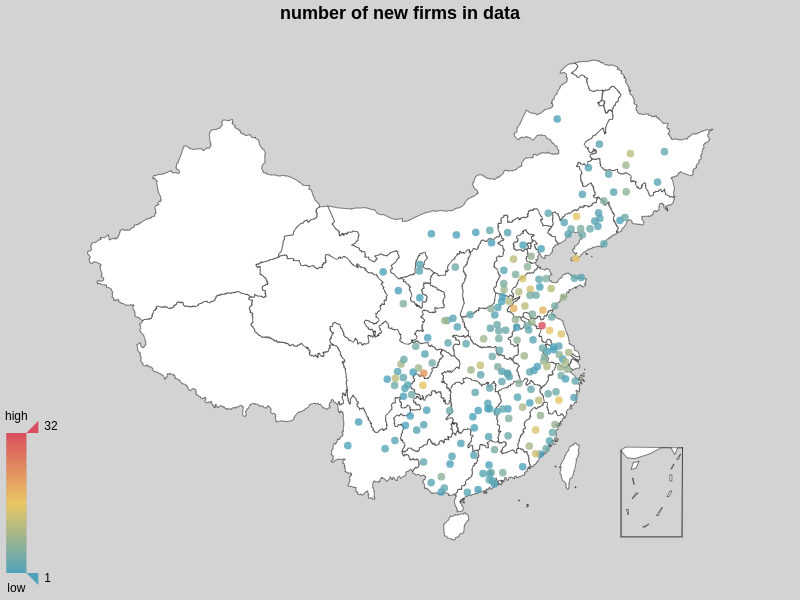
\includegraphics[scale=0.4]{\graphs/number of new firms in data.png}
    \label{firm_city_map}
    \fnote{Notes: Each point in the map represents a city which
        lands at least one firm in my data set, and
        there are 213 such cities in my data set.
        The color of the point denotes the number of firms a city lands,
        and the number increases as the color changes from blue to red.}
\end{figure}





I also show the descriptive statistics of the variables used for estimation in \Cref{table: descriptive statistics}:
\begin{table}[H]
\centering
\caption{Descriptive statistics of firm level variables and city wage}
\label{table: descriptive_statistics}
\begin{tabular}{cccccc}
\toprule
 & land price (1,000 yuan/hectare) & output (1,000 yuan) & number of workers (person) & area of land (hectare) & city wage (1,000 yuan/year) \\
\midrule
mean & 1685.10 & 170733.30 & 228.16 & 4.59 & 35.96 \\
std & 934.95 & 409499.05 & 143.57 & 5.65 & 8.24 \\
min & 379.50 & 5662.00 & 10.00 & 0.03 & 17.21 \\
25% & 978.62 & 38354.00 & 125.00 & 1.60 & 30.49 \\
50% & 1440.01 & 72909.00 & 223.00 & 2.83 & 34.62 \\
75% & 2015.52 & 164553.00 & 324.50 & 5.40 & 39.81 \\
max & 6001.56 & 7282607.00 & 2326.00 & 65.48 & 77.03 \\
N & 1019.00 & 1019.00 & 1019.00 & 1019.00 & 288.00 \\
\bottomrule
\end{tabular}
\end{table}


\Cref{distribution of output and price} shows
the distribution of land price and firms' output level,
which are the two most important variables in my model.

\begin{figure}[H]
    \centering
    \caption{Sample distribution of output level and land price}
    \resizebox{\columnwidth}{!}{
        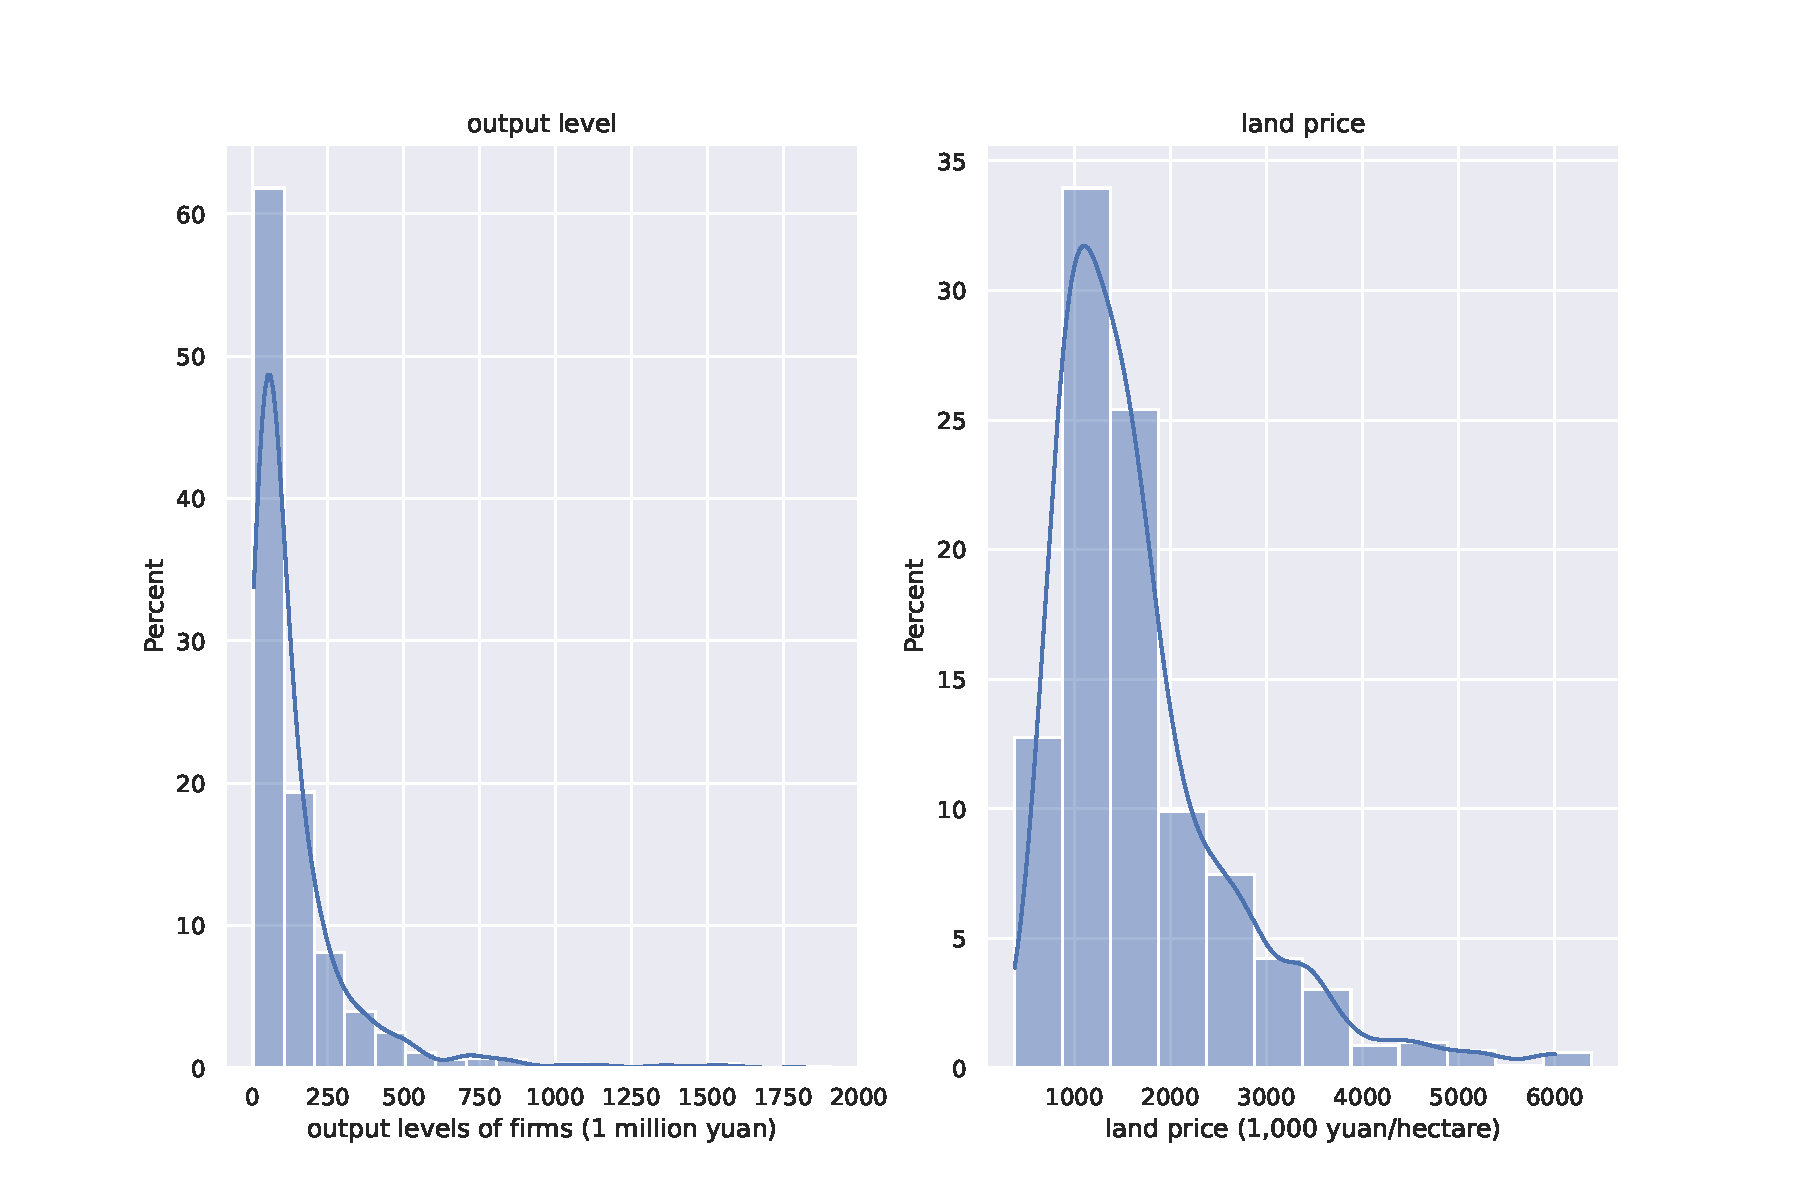
\includegraphics{\graphs/data_distribution.pdf}
    }
    \fnote{Notes: The blue line in the graphs are kernel density plots.
        To make the first histogram clearer, I just draw the
        distribution of firms with output levels smaller than 2 billion yuan/year. There
        are several firms with output levels of more than 2 billion yuan/year, which makes the
        actual tail of the distribution of output fatter.}
    \label{distribution of output and price}
\end{figure}

According to \Cref{distribution of output and price},
both the distributions of the output level of firms and the industrial land price are left-skewed,
moreover, more than 80\% firms have output levels between 5 million
and 250 million yuan per year, and most of the firms buy land with a price below 3 million yuan per
hectare. This implies most of the industrial land is sold at relatively low prices in my data set,
which is consistent with my observations in \Cref{sec:intro} and \Cref{sec:institution}.


